
\subsection{The Theory of Hurricanes}
\label{sec:hurr-theory}
\subsubsection{The Carnot cyclone}
\label{sec:carnot}

The hurricane can be idealised as a Carnot cycle as in Figure~\ref{fig:hurricane-carnot},
as was originally proposed Kleinschmidt,~1951~\cite{kleinschmidt1951grundlagen},
and reproposed by Emanuel~1986~\cite{emanuel1986air, emanuel1987dependence, lilly1985steady,}.
\begin{figure}
\centering
    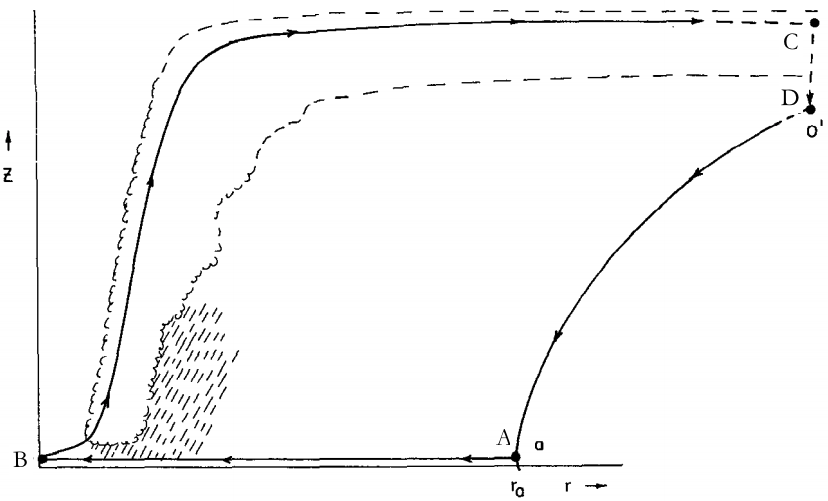
\includegraphics[width=\linewidth]{images/hurricane-carnot.png}\\
    \textit{Figure 1 from~\cite{emanuel1991theory}. }
    \caption{An idealised Carnot cycle where air parcels travel clockwise:
            A$\rightarrow$B travelling isothermally inwards into the eye-wall extracting enthalpy
            from the sea, and gaining entropy through kinetic energy dissipation;
            B$\rightarrow$C moist adiabatically thrust up into the stratosphere
            at the eye-wall and out to some some subsidence point;
            C$\rightarrow$D initial isothermal descent, albeit with some loss through radiation;
            D$\rightarrow$A final moist adiabatic descent~\cite{emanuel2018progress}. }
            \label{fig:hurricane-carnot}

\end{figure}


Hurricanes are a finite amplitude instability, and there is a
clear separation between a tropical storm and a hurricane~\cite{emanuel2005divine}.

As shown in Figure~\ref{fig:hurricane-carnot} Enthalpy is acquired from the sea surface,
and entropy from the dissipation of kinetic energy,
 as the air travels isothermally towards the eyewall.
 At the eyewall the air rises moist adiabatically
 to the lower stratosphere and out to some distance from the storm.
 In a simplified model it then subsides
 approximately isothermally at first, albeit with some loss through radiation.
 The final descent is approximately moist adiabatic~\cite{emanuel2018progress}.

This is nearly an ideal carnot cycle, this converts heat energy of the sea surface into
mechanical energy of the winds, doing the majority of the work against the sea surface.

The potential intensity (equation 15-7 in \cite{emanuel2018progress}) is,

\begin{equation}
\left|\mathbf{V}_{s}\right|^{2}=\frac{C_{k}}{C_{D}} \frac{T_{s}-T_{o}}{T_{o}}\left(k_{0}^{*}-k\right),
\tag{PI}
\label{eq:PI}
\end{equation}

where $C_d$ is the surface drag coefficient $C_k$ is the dimensionless
surface exchange coefficient for enthalpy.
$T_s$ is the sea surface temperature, $T_o$ is the temperature of the
lower stratosphere at the end of the moist adiabatic rise.
One can see that the a warmer sea surface, and a cooler lower stratosphere
would both lead to a higher potential intensity in paragraph~\cite{emanuel1991theory, emanuel2018progress}.
Further in \ref{eq:PI} the enthalpy per unit mass (equation 15-8 in \cite{emanuel2018progress}) is

\begin{equation}
k \equiv c_{p} T+L_{v} q,
\label{eq:enthalpy_per_unit_mass}
\end{equation}

where $c_p$ is the heat capacity at constant pressure and $L_{v}$ is the latent heat
of vaporisation. $k_{0}^{*}$ is the saturation enthalpy at the sea surface.


There is a positive feedback loop from air cooling adiabatically as it flows down
the pressure gradient, and therefore increasing the enthalpy disequilibrium
$k_{0}^{*}-k$, leading to a root below 700 mbar central pressure called a `hypercane'.


To explore the impact that an increased amount of greenhouse gasses might have
on the system, consider a single layer model of the atmosphere, described by the
set of four simultanious equations.

\begin{eqnarray}
F_{\mathrm{solar}} =& F_{\mathrm{atm}} + F_{\mathrm{ground}}\tau_{\mathrm{IR}}\\
F_{\mathrm{solar}}(1-\tau_{\mathrm{vis}}) =& 2F_{\mathrm{atm}} + F_{\mathrm{ground}}(\tau_{\mathrm{IR}}-1)\\
F_{\mathrm{solar}}(\tau_{\mathrm{vis}}) +F_{\mathrm{atm}} =&F_{\mathrm{ground}} \\
\sigma T_{\mathrm{ground}}{}^4 =& F_{\mathrm{ground}}
\end{eqnarray}

which leads to the solution

\begin{equation}
T_{\mathrm{ground}} = \left( \frac{F_{\mathrm{solar}}}{\sigma}\frac{(1+\tau_{\mathrm{vis}})}{(1+\tau_{\mathrm{IR}})}\right)^{1/4}
\end{equation}

which shows that when $\tau_{\mathrm{IR}}$, i.e.~the ammount of greenhouse gasses,
is increased, this leads to an increase in the temperature of the (sea) surface (c. $T_s$).
When using the Stefan-Boltzmann relation,

\begin{equation}
F_{\mathrm{atm}} = \sigma T_a{}^{4},
\end{equation}

we can further find that the

\begin{equation}
T_{\mathrm{atm}}^{4}=T_{\mathrm{ground}}^4\frac{(1-\tau_{\mathrm{vis}}\tau_{\mathrm{IR}})}{(1+\tau_{vis})}
\end{equation}

so that the temperature of the atmosphere (approximately equivalent to $T_{o}$)
decreases as the amount of greenhouse gases are increased.


One can then use \ref{eq:PI} and see that as the nominator has increased, and the
denominator has decreased, the potential intensity is expected to increase with the
ammount of greenhouse gases, $\tau_IR$, in the atmosphere.


Bister 2002 gives an algorithm whereby given the rest of the climate
there is some maximum intensity that a hurricane could reach  \cite{bister2002low}.
This is a development of the original work~\cite{bister1996development,bister1998dissipative, bister2002low}

This makes some simplifying assumptions. One of the main reasons for
hurricanes failing to reach their potential intensity is that not all of the
water column at the temperature
of the surface, instead only up to some depth. The depth of warm water
is much larger at the western boundary currents~\cite{hogg1995western}, which means that if a hurricane
travels down the axis of the current (e.g. the loop current)
it can reach a higher intensity than
if it travelled 20km to one side.


A few super-intense tropical cyclones have been observed, although this is still a
matter of some dispute, and the community still trusts the assumptions made in the
Carnot cyclone model~\cite{camargo2019tropical}.




\subsubsection{Cyclogenesis}


Given that there is a thermodynamic disequilibrium between the Ocean and
atmosphere, it is reasonable to ask why there are not more tropical cyclones
continuously spontaniously emerging. Cyclogenesis is one of the
 great mysteries of the tropical atmosphere~\cite{emanuel2005divine}.

Warm air rises in cumulonimbus clouds,
 dries, and then falls down very dry.
A decrease in humidity with altitude.
 Middle level dryness.
cumulonimbus clouds clump together.
 More updrafts give more rain.
Nascent cloud cluster dies away.
Middle atmosphere becomes humidified.

William Grey made the first comprehensive study of cyclogenesis in 1975~\cite{gray1975tropical},
showing that there were a number of diverse phenomena that triggered the growth of TC.
In the North Atlantic, the primary trigger seems to be the passage of African Easterly Waves,
that sometimes deepen into tropical depressions and then hurricanes. Cyclogenesis can also be caused by an Ordinary cold front that penetrates tropics,
providing the same nucleation. There was a tropical cold bias in CMIP5 models~\cite{camargo2013global},
possibly caused by the way moisture was dealt with by CMIP models~\cite{seager2019strengthening},
and this could have caused the under observation of tropical cyclones in those models.
African easterly waves are also relatively difficult to resolve.



In contrast to this EC does not need anything to trigger it, forming
spontaniously through the baroclinic instability in the extratropical atmosphere~\cite{lorenz1960energy}.
This is one reason as to why extratropical cyclones seem to come in a continuous spectrum,
whereas tropical cyclones seem to have a clear break between tropical storms and cyclones.
Extratropical cyclones must reasonably also have some maximum size that they can be
expected to reach given the climate, but given that they cause significantly less damage
and smaller storm surges, and no theory has been set out to suggest what this might be,
they will be largely ignored in the rest of this thesis.




\begin{figure*}
\centering
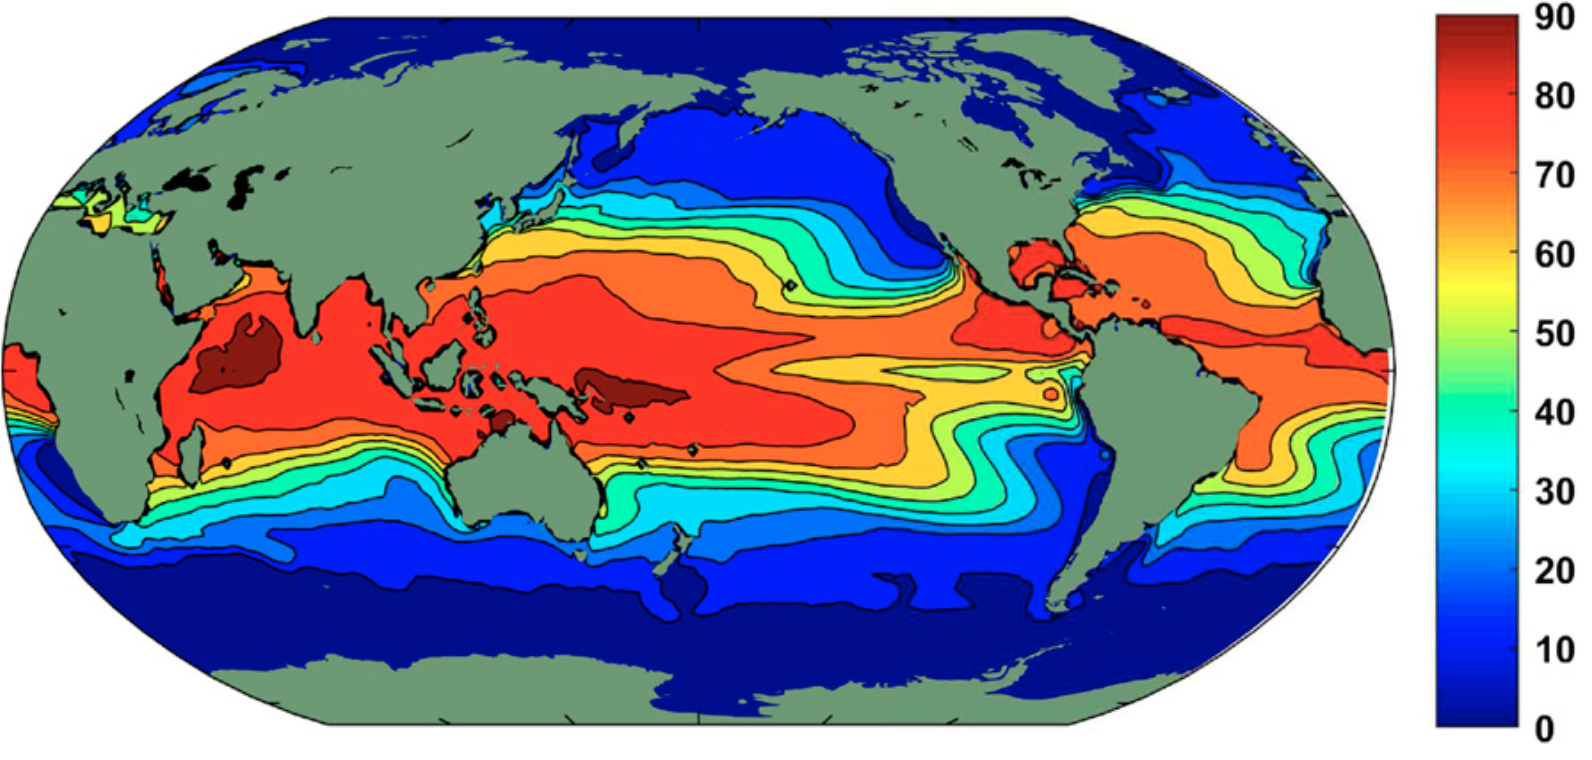
\includegraphics[width=\linewidth]{images/PI-max-year.png}\\
\textit{Figure 15-7 from \cite{emanuel2018progress}.}
\caption{The annual maximum of the potential intensity (m s$^{-1}$), calculated using
~\cite{bister2002low} and ERA-Interim data 1979-2016.
This is product maps on well to the block maxima procedure in §~\ref{sec:evt}.
}
\label{fig:eman}
\end{figure*}

